\documentclass{article}
\usepackage[utf8]{inputenc}
\usepackage[T1]{fontenc}
\usepackage[portuguese]{babel}
\usepackage{geometry}
\geometry{a4paper, margin=1in}

\usepackage{amsmath}
\usepackage{amssymb}
\usepackage{amsthm}
\usepackage{algorithm}
\usepackage{algpseudocode}
\usepackage{enumitem}
\usepackage{booktabs}
\usepackage{float}
\usepackage{listings}
\usepackage{xcolor}
\usepackage{graphicx}

% --- Definições de comandos personalizados ---
\newcommand{\R}{\mathbb{R}}
\newcommand{\T}{^{\top}}
\newcommand{\burden}[1]{\textsf{\footnotesize[#1]}}

% --- Ambientes matemáticos ---
\newtheorem{teorema}{Teorema}
\newtheorem{proposicao}{Proposição}
\theoremstyle{remark}
\newtheorem{obs}{Observação}

% --- Configurações de código ---
% Caracteres acentuados dentro de lstlisting precisam ser mapeados explicitamente
% (sem isso o pacote listings falha com UTF-8 ou "come" o espaço após o acento).
\lstset{
    language=Python,
    basicstyle=\ttfamily\footnotesize,
    keywordstyle=\color{blue},
    stringstyle=\color{orange},
    commentstyle=\color{green!60!black},
    numbers=left,
    numberstyle=\tiny\color{gray},
    stepnumber=1,
    breaklines=true,
    frame=single,
    showstringspaces=false,
    inputencoding=utf8,
    extendedchars=true,
    literate=
      {á}{{\'a}}1 {é}{{\'e}}1 {í}{{\'i}}1 {ó}{{\'o}}1 {ú}{{\'u}}1
      {â}{{\^a}}1 {ê}{{\^e}}1 {ô}{{\^o}}1
      {ã}{{\~a}}1 {õ}{{\~o}}1 {Ã}{{\~A}}1
      {ç}{{\c c}}1
      {—}{{\textemdash}}1 {–}{{\textendash}}1
      {ª}{{\textordfeminine}}1 {±}{{\ensuremath{\pm}}}1 {§}{{\S}}1
}

\begin{document}

\title{Resolução da Lista 2 - Métodos numéricos}
\author{Larissa de Souza e Otávio Menezes}
\date{05/10/2026}
\maketitle

\section*{Convenções e referências}
As referências do tipo \burden{Teorema 6.21, p.~458} remetem a R.~L.~Burden, J.~D.~Faires e A.~M.~Burden,
\emph{Análise Numérica}, 10\textordfeminine{} ed., Cengage Learning (tradução brasileira). A Questão~3 segue a Seção~10.11
de H.~Anton e C.~Rorres, \emph{Álgebra Linear com Aplicações}. Seguindo o livro \burden{Definição 6.22, p.~459}, uma matriz
$A\in\R^{n\times n}$ é \textbf{positiva definida} (PD) quando é simétrica e $x\T Ax>0$ para todo $x\neq0$. Para cada linha $i$,
denotamos $R_i=\sum_{j\ne i}|a_{ij}|$ (soma dos módulos fora da diagonal).

\paragraph{Implementação.} Cada questão tem um arquivo próprio (\texttt{questao1.py}, \dots, \texttt{questao4.py}),
reproduzidos no Apêndice. Conforme as instruções da lista, \emph{nenhuma} rotina pronta de álgebra linear foi usada
(nada de \texttt{numpy.linalg} ou \texttt{scipy}): o NumPy serve apenas como contêiner de vetores/matrizes e para
operações elementares (somas, produtos escalares, produto externo, operações entre linhas). Todos os algoritmos
(eliminação, fatorações, substituições) estão escritos explicitamente. Como as operações vetorizadas do NumPy executam em C,
os tempos absolutos da Questão~2 refletem também essa escolha, mas os três métodos usam as mesmas primitivas.

%==========================================================================
\section{Questão 1 --- Gerador de matrizes positivas definidas}
%==========================================================================

\subsection{Ideia}
O teorema do enunciado diz que basta construir uma matriz que seja, \emph{ao mesmo tempo},
(i) simétrica, (ii) estritamente diagonal dominante \burden{Definição 6.20, p.~457}, isto é,
$|a_{ii}|>R_i$ para todo $i$, e (iii) com diagonal não-negativa. As três propriedades podem ser
\emph{impostas por construção}: sorteamos livremente a parte fora da diagonal (de forma simétrica) e, só depois,
escolhemos cada $a_{ii}$ maior que a soma $R_i$ já sorteada.

\begin{algorithm}[H]
\caption{\texttt{gerar\_matriz\_pd}$(n)$}
\begin{algorithmic}[1]
\Require dimensão $n$
\Ensure $A\in\R^{n\times n}$ positiva definida
\For{$i=2,\dots,n$}
  \For{$j=1,\dots,i-1$}
    \State sorteie $a_{ij}\sim\mathcal U(-1,1)$ e faça $a_{ji}\gets a_{ij}$ \Comment{simetria}
  \EndFor
\EndFor
\For{$i=1,\dots,n$}
  \State sorteie $\delta_i\sim\mathcal U(1,2)$ \Comment{folga estritamente positiva}
  \State $a_{ii}\gets R_i+\delta_i=\sum_{j\ne i}|a_{ij}|+\delta_i$
\EndFor
\State \Return $A$
\end{algorithmic}
\end{algorithm}

\subsection{Por que \emph{toda} matriz gerada é positiva definida}
Por construção:
\begin{enumerate}[label=(\roman*)]
  \item $a_{ji}=a_{ij}$, logo $A=A\T$;
  \item $a_{ii}=R_i+\delta_i>R_i$ com $\delta_i\ge 1>0$, logo $A$ é estritamente diagonal dominante;
  \item $a_{ii}=R_i+\delta_i\ge 1>0$, logo a diagonal é positiva (em particular não-negativa).
\end{enumerate}
As hipóteses do teorema são satisfeitas para \emph{qualquer} sorteio, portanto $A$ é PD. Para deixar a
justificativa completa, mostramos também o teorema, com uma estimativa quantitativa.

\begin{teorema}\label{teo:sdd}
Se $A$ é simétrica, estritamente diagonal dominante e $a_{ii}\ge 0$, então para todo $x\in\R^n$
\[
   x\T A x \;\ge\; \min_i\,(a_{ii}-R_i)\;\|x\|_2^2 ,
\]
e, como $\min_i(a_{ii}-R_i)>0$, $A$ é positiva definida.
\end{teorema}
\begin{proof}
Da dominância estrita, $|a_{ii}|>R_i\ge 0$; como $a_{ii}\ge0$, temos $a_{ii}=|a_{ii}|>R_i$.
Expandindo a forma quadrática e usando $x_ix_j\ge -|x_i||x_j|$:
\[
x\T A x=\sum_i a_{ii}x_i^2+\sum_{i\neq j}a_{ij}x_ix_j
\;\ge\;\sum_i a_{ii}x_i^2-\sum_{i\neq j}|a_{ij}|\,|x_i|\,|x_j|.
\]
Pela desigualdade $|x_i||x_j|\le\tfrac12(x_i^2+x_j^2)$ e pela simetria ($|a_{ij}|=|a_{ji}|$),
\[
\sum_{i\neq j}|a_{ij}|\,|x_i|\,|x_j|\le \frac12\sum_{i\ne j}|a_{ij}|x_i^2+\frac12\sum_{i\ne j}|a_{ji}|x_j^2
=\sum_i x_i^2\sum_{j\ne i}|a_{ij}| = \sum_i R_i\,x_i^2 .
\]
Logo $x\T Ax\ge\sum_i (a_{ii}-R_i)x_i^2\ge \min_i(a_{ii}-R_i)\,\|x\|_2^2$, que é $>0$ se $x\neq0$.
\end{proof}

\paragraph{Outras duas justificativas, usando apenas resultados do livro.}
\begin{itemize}
\item \textbf{Via autovalores.} Pelo Teorema do Círculo de Geršgorin \burden{Teorema 9.1, p.~626}, todo autovalor
$\lambda$ de $A$ pertence a algum disco $\{z:|z-a_{ii}|\le R_i\}$. Como $A$ é simétrica, seus autovalores são reais
\burden{Corolário 9.17, p.~639}; então $\lambda\ge a_{ii}-R_i=\delta_i\ge1>0$. Uma matriz simétrica com todos os
autovalores positivos é PD \burden{Teorema 9.18, p.~639}.
\item \textbf{Via eliminação de Gauss.} Matrizes estritamente diagonal dominantes admitem eliminação de Gauss
\emph{sem trocas de linhas} e cada matriz reduzida continua estritamente diagonal dominante
\burden{Teorema 6.21, p.~458}. Com diagonal positiva, cada novo pivô satisfaz
$a^{(2)}_{jj}=a_{jj}-\frac{a_{j1}a_{1j}}{a_{11}}\ge a_{jj}-|a_{j1}|\frac{|a_{1j}|}{a_{11}}>a_{jj}-|a_{j1}|>0$
(a última desigualdade vale porque $a_{jj}>R_j\ge|a_{j1}|$). Assim, todos os pivôs são positivos e, pelo
\burden{Teorema 6.26, p.~463}, a matriz simétrica $A$ é PD.
\end{itemize}

\begin{obs}
Escolher $\delta_i\in[1,2)$ (e não apenas $\delta_i>0$) garante, pela estimativa acima, que o menor autovalor é
$\ge 1$. Isso evita matrizes quase singulares e mantém o condicionamento bom, o que é desejável no experimento
da Questão~2 com $n$ até $500$.
\end{obs}

\subsection{Três exemplos gerados (\texttt{questao1.py}, semente 2026)}
Para cada exemplo, o programa verifica simetria, dominância diagonal estrita e diagonal não-negativa,
calcula a folga $\min_i(a_{ii}-R_i)$ e, como teste empírico, o menor valor de $x\T Ax/x\T x$ entre
$20\,000$ vetores aleatórios. Pelo Teorema~\ref{teo:sdd}, este último deve ser $\ge$ folga.

\[
A_1=\begin{bmatrix}
2.2925 & -0.6421 & 0.2798 \\
-0.6421 & 2.0625 & -0.0655 \\
0.2798 & -0.0655 & 2.1358
\end{bmatrix}
\qquad
A_2=\begin{bmatrix}
3.1459 & -0.9081 & 0.8514 & -0.2326 \\
-0.9081 & 3.4099 & -0.4378 & 0.4900 \\
0.8514 & -0.4378 & 3.2717 & -0.4743 \\
-0.2326 & 0.4900 & -0.4743 & 2.3351
\end{bmatrix}
\]
\[
A_3=\begin{bmatrix}
4.1529 & -0.2612 & -0.9034 & -0.9409 & 0.8354 \\
-0.2612 & 2.2808 & -0.0447 & -0.0015 & 0.3924 \\
-0.9034 & -0.0447 & 3.7508 & -0.8454 & 0.4409 \\
-0.9409 & -0.0015 & -0.8454 & 4.0634 & -0.4299 \\
0.8354 & 0.3924 & 0.4409 & -0.4299 & 3.2997
\end{bmatrix}
\]

\begin{table}[H]\centering\small
\begin{tabular}{@{}lccccc@{}}\toprule
 & simétrica & estr. diag. dom. & $a_{ii}\ge0$ & $\min_i(a_{ii}-R_i)$ & $\min x\T Ax/x\T x$ (empírico)\\\midrule
$A_1$ ($3\times3$) & sim & sim & sim & 1.3549 & 1.4968\\
$A_2$ ($4\times4$) & sim & sim & sim & 1.1382 & 1.9436\\
$A_3$ ($5\times5$) & sim & sim & sim & 1.2012 & 1.7381\\\bottomrule
\end{tabular}
\caption{Verificações dos exemplos. Por exemplo, em $A_1$: $R=(0.9220,\,0.7076,\,0.3453)$ e
$\operatorname{diag}(A_1)=(2.2925,\,2.0625,\,2.1358)$.}
\end{table}

%==========================================================================
\section{Questão 2 --- Eliminação de Gauss, $P\T LU$ e Cholesky}
%==========================================================================

\subsection{Substituições (progressiva e regressiva)}
Os três métodos terminam em sistemas triangulares.
\begin{itemize}
\item \textbf{Substituição regressiva} ($Ux=y$, $U$ triangular superior) \burden{Algoritmo 6.1, passos 8--9, p.~403}:
\[
x_n=\frac{y_n}{u_{nn}},\qquad x_i=\frac{1}{u_{ii}}\Big(y_i-\sum_{j=i+1}^{n}u_{ij}x_j\Big),\quad i=n-1,\dots,1.
\]
\item \textbf{Substituição progressiva} ($Ly=b$, $L$ triangular inferior) \burden{p.~450--451}:
\[
y_1=\frac{b_1}{l_{11}},\qquad y_i=\frac{1}{l_{ii}}\Big(b_i-\sum_{j=1}^{i-1}l_{ij}y_j\Big),\quad i=2,\dots,n,
\]
com $l_{ii}=1$ (sem divisão) no caso de Doolittle.
\item \textbf{Regressiva com a transposta} ($L\T x=y$, usada no Cholesky) \burden{passos 9--10, p.~466}: como
$(L\T)_{ij}=l_{ji}$, não é preciso montar $L\T$:
\(
x_i=\frac{1}{l_{ii}}\big(y_i-\sum_{j=i+1}^{n}l_{ji}x_j\big).
\)
\end{itemize}
Cada substituição custa $\approx n^2/2$ multiplicações e $\approx n^2/2$ adições, isto é, $O(n^2)$.

\subsection{Eliminação de Gauss com pivoteamento parcial com escala}
A eliminação transforma $[A\,|\,b]$ numa matriz triangular superior com as operações
$(E_j-m_{ji}E_i)\to(E_j)$, $m_{ji}=a^{(i)}_{ji}/a^{(i)}_{ii}$ \burden{Seção 6.1, p.~396--403}.
Um pivô pequeno em relação aos demais elementos amplifica erros de arredondamento
(exemplo do pivô $0{,}003$ em \burden{Seção 6.2, p.~411--413}). O \textbf{pivoteamento parcial com escala}
\burden{Algoritmo 6.3, p.~416--417} compara os candidatos \emph{relativamente} ao tamanho de suas linhas:
\begin{enumerate}
\item fatores de escala, calculados \emph{uma única vez}: $s_i=\max_{1\le j\le n}|a_{ij}|$ (se algum $s_i=0$, não há solução única);
\item na etapa $i$, escolhe-se o menor $p\ge i$ tal que
\(\displaystyle \frac{|a_{pi}|}{s_p}=\max_{i\le k\le n}\frac{|a_{ki}|}{s_k}\)
e troca-se $(E_i)\leftrightarrow(E_p)$;
\item eliminação: $m_{ji}=a_{ji}/a_{ii}$ e $E_j\gets E_j-m_{ji}E_i$, $j>i$; ao final, substituição regressiva.
\end{enumerate}
Como no livro, as trocas são \emph{simuladas} com o vetor \texttt{NLINHA} (só índices são trocados).
\textbf{Custo:} $\frac{n^3}{3}+n^2-\frac n3$ multiplicações/divisões e $\frac{n^3}{3}+\frac{n^2}{2}-\frac{5n}{6}$
adições/subtrações \burden{p.~406--407}; a escala acrescenta apenas $\frac32n(n-1)$ comparações e
$\frac{n(n+1)}{2}-1$ divisões \burden{Eq.~(6.7), p.~419}, ou seja, $O(n^2)$.
\textbf{Ponto crucial para o item (b):} a eliminação opera sobre $[A\,|\,b]$; para um novo $b$, todo o trabalho
$O(n^3/3)$ precisa ser refeito.

\subsection{Decomposição $P\T LU$}
Se a eliminação pode ser feita sem trocas, então $A=LU$, com $L$ triangular inferior unitária formada pelos
multiplicadores $m_{ji}$ e $U$ a matriz triangular final \burden{Teorema 6.19, p.~448}. Havendo trocas, existe uma
matriz de permutação $P$ (identidade com linhas reordenadas) tal que $PA=LU$; como $P^{-1}=P\T$,
\[
A=P\T LU \qquad\burden{p.~451--452}.
\]
\textbf{Cálculo de $L$ e $U$} (forma de Doolittle, $l_{ii}=1$) \burden{Algoritmo 6.4, p.~450}: igualando as entradas de
$PA=LU$,
\[
u_{ij}=a_{ij}-\sum_{k=1}^{i-1}l_{ik}u_{kj}\ (j\ge i),\qquad
l_{ji}=\frac{1}{u_{ii}}\Big(a_{ji}-\sum_{k=1}^{i-1}l_{jk}u_{ki}\Big)\ (j>i).
\]
Na etapa $i$, antes de dividir por $u_{ii}$, calculam-se os candidatos $a_{ji}-\sum_k l_{jk}u_{ki}$ ($j\ge i$),
que são exatamente os valores $a^{(i)}_{ji}$ da eliminação, e escolhe-se o pivô pelo \emph{mesmo} critério com
escala; a troca de linhas é registrada no vetor \texttt{perm}, que representa $P$.
\textbf{Resolução:} $Ax=b\iff LUx=Pb$; resolve-se $Ly=Pb$ (progressiva) e $Ux=y$ (regressiva).
\textbf{Custo:} fatoração $O(n^3/3)$ (a mesma da eliminação), mas cada novo $b$ custa apenas $O(2n^2)$
\burden{Seção 6.5, p.~445--446}: ``uma vez que a fatoração esteja determinada, os sistemas envolvendo a matriz $A$
podem ser resolvidos desta maneira simplificada para qualquer número de vetores $b$''.

\subsection{Decomposição de Cholesky}
Pelo \burden{Corolário 6.28, p.~463}, $A$ é PD se e somente se $A=LL\T$ com $L$ triangular inferior de
diagonal não nula. Igualando as entradas de $A=LL\T$ (para $j\ge i$, $a_{ji}=\sum_{k=1}^{i}l_{jk}l_{ik}$) e isolando
o termo $k=i$, obtêm-se as fórmulas do \burden{Algoritmo 6.6, p.~464}:
\[
l_{ii}=\sqrt{a_{ii}-\sum_{k=1}^{i-1}l_{ik}^2},\qquad
l_{ji}=\frac{1}{l_{ii}}\Big(a_{ji}-\sum_{k=1}^{i-1}l_{jk}l_{ik}\Big),\quad j=i+1,\dots,n.
\]
\textbf{Resolução:} $Ly=b$ (progressiva) e $L\T x=y$ (regressiva com a transposta).
\textbf{Por que não precisa de pivoteamento:} para $A$ simétrica PD, a eliminação sem trocas tem todos os pivôs
positivos e é estável em relação ao crescimento de erros de arredondamento \burden{Teorema 6.26, p.~463}.
\textbf{Custo:} $\frac{n^3}{6}+\frac{n^2}{2}-\frac{2n}{3}$ multiplicações/divisões e $\frac{n^3}{6}-\frac n6$
adições/subtrações, mais $n$ raízes quadradas \burden{p.~465} --- \emph{metade} do custo de $LU$, porque a simetria
permite calcular só a metade inferior.

\paragraph{Aplicabilidade.} As matrizes do experimento vêm da Questão~1, logo são PD. Então $A$ é invertível
\burden{Teorema 6.23(i), p.~460}, de modo que a eliminação e a fatoração $P\T LU$ existem, e a fatoração de Cholesky
existe pelo Corolário~6.28. Os três métodos produzem a mesma solução; o programa confere o resíduo
$\|Ax-b\|_\infty$, que ficou abaixo de $5\times10^{-14}$ em todos os sistemas.

\subsection{Desenho do experimento e previsão teórica}
\begin{itemize}
\item \textbf{(a)} Para cada $n$, 10 pares $(A_k,b_k)$ com $A_k$ distintas: cada método processa cada $A_k$ do zero.
\item \textbf{(b)} Para cada $n$, uma única $A$ e 10 vetores $b_k$: Gauss refaz a eliminação 10 vezes, enquanto
$P\T LU$ e Cholesky \textbf{fatoram uma única vez} e reutilizam os fatores, repetindo apenas as substituições.
\end{itemize}
Contando apenas os termos dominantes (multiplicações):
\begin{table}[H]\centering
\begin{tabular}{@{}lccc@{}}\toprule
 & Gauss (escala) & $P\T LU$ & Cholesky\\\midrule
(a) 10 matrizes & $10\cdot\frac{n^3}{3}$ & $10\big(\frac{n^3}{3}+n^2\big)$ & $10\big(\frac{n^3}{6}+n^2\big)$\\
(b) 1 matriz, 10 vetores & $10\cdot\frac{n^3}{3}$ & $\frac{n^3}{3}+10n^2$ & $\frac{n^3}{6}+10n^2$\\\bottomrule
\end{tabular}
\caption{Custo teórico aproximado.}
\end{table}
\noindent Previsão pela contagem de operações: em (a), Cholesky $\approx$ metade de $P\T LU$, e Gauss $\approx P\T LU$ (mesmo número de operações);
em (b), $P\T LU$ e Cholesky muito mais rápidos que Gauss (razão $\to10$ ou mais quando $n$ cresce), e Cholesky ainda à frente.

\paragraph{Medição.} Tempo de parede (\texttt{time.perf\_counter}) só da resolução (a geração das matrizes não
entra). Cada tempo total (10 sistemas) foi medido 5 vezes e foi registrada a mediana, para reduzir o ruído do
sistema operacional.

\subsection{Resultados}
\begin{table}[H]\centering
\begin{tabular}{@{}r|ccc|ccc@{}}\toprule
 & \multicolumn{3}{c|}{(a) 10 matrizes distintas (s)} & \multicolumn{3}{c}{(b) 1 matriz, 10 vetores (s)}\\
$n$ & Gauss & $P\T LU$ & Cholesky & Gauss & $P\T LU$ & Cholesky\\\midrule
100 & 0.0228 & 0.0115 & \textbf{0.0078} & 0.0191 & 0.0034 & \textbf{0.0031}\\
200 & 0.0797 & 0.0296 & \textbf{0.0186} & 0.0658 & 0.0074 & \textbf{0.0060}\\
300 & 0.3348 & 0.0501 & \textbf{0.0290} & 0.2586 & 0.0119 & \textbf{0.0097}\\
400 & 1.0065 & 0.0814 & \textbf{0.0498} & 0.8774 & 0.0170 & \textbf{0.0141}\\
500 & 1.8321 & 0.1111 & \textbf{0.0592} & 1.8261 & 0.0227 & \textbf{0.0179}\\\bottomrule
\end{tabular}
\caption{Tempo total de execução (em segundos, para os 10 sistemas) por método e por $n$. Os valores absolutos
dependem da máquina; o que importa é a relação entre os métodos.}
\end{table}

\begin{figure}[H]\centering
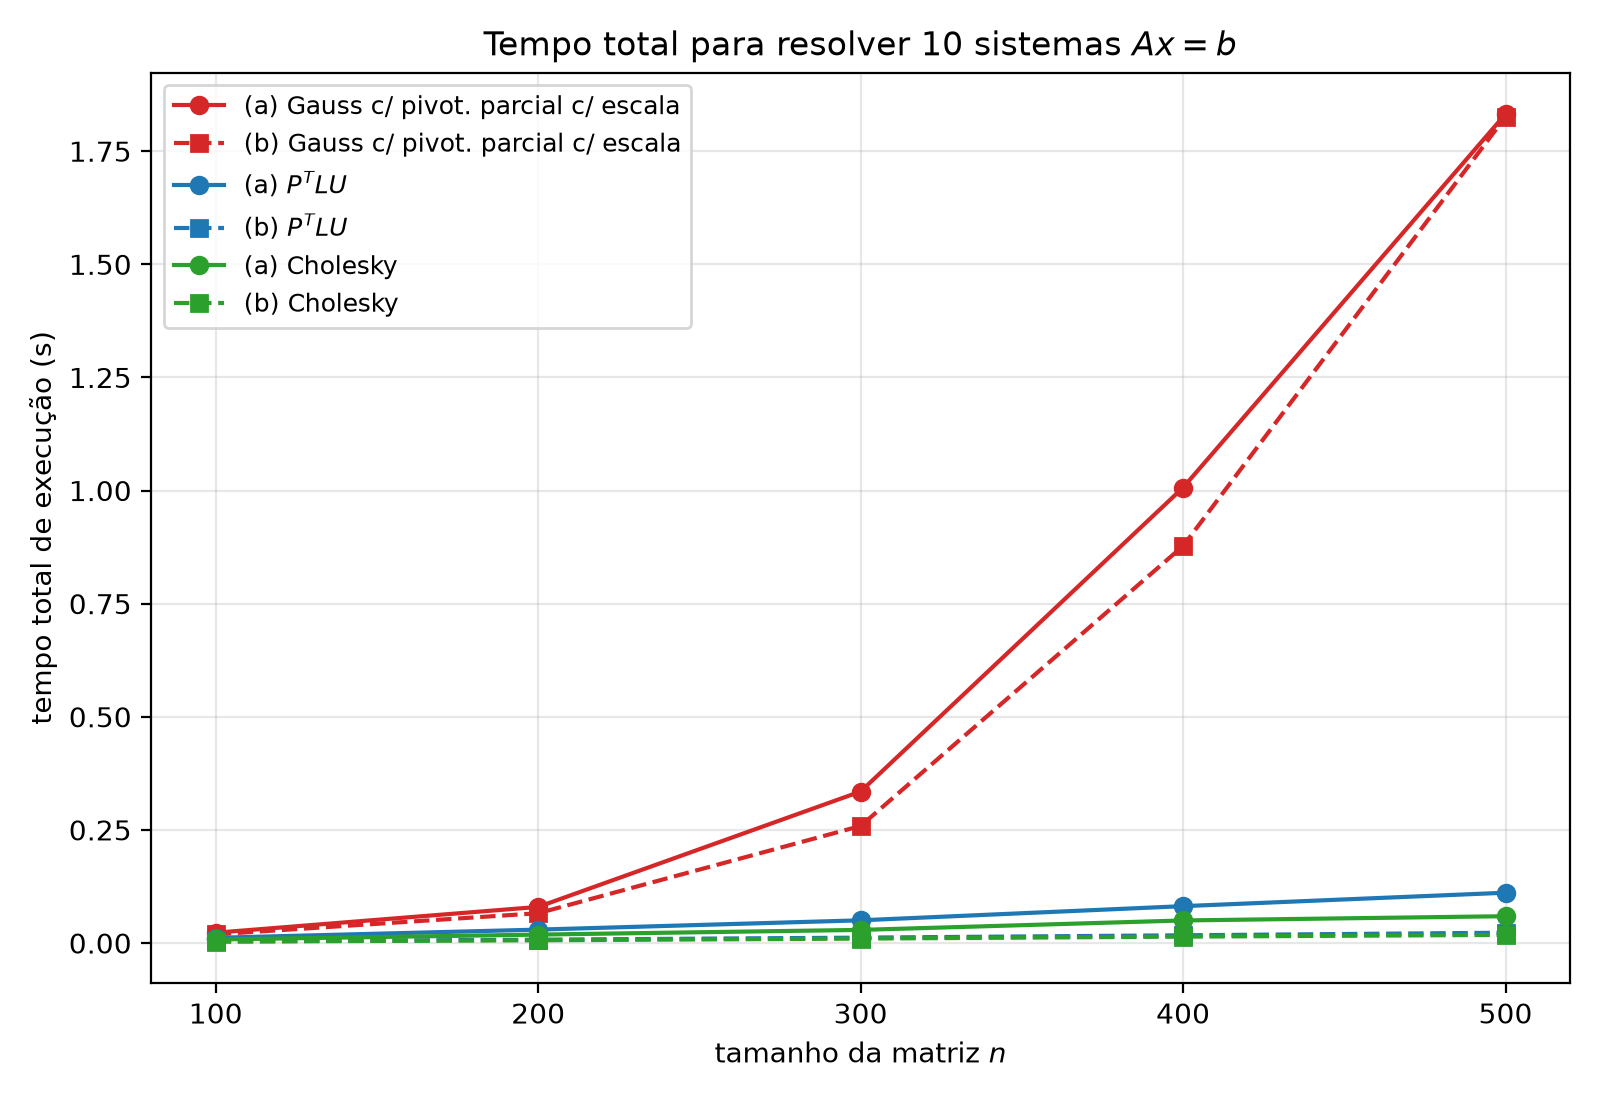
\includegraphics[width=0.82\textwidth]{q2_tempos.png}
\caption{As 6 curvas de tempo $\times$ $n$. Linhas cheias: item (a); tracejadas: item (b).}
\end{figure}
\begin{figure}[H]\centering
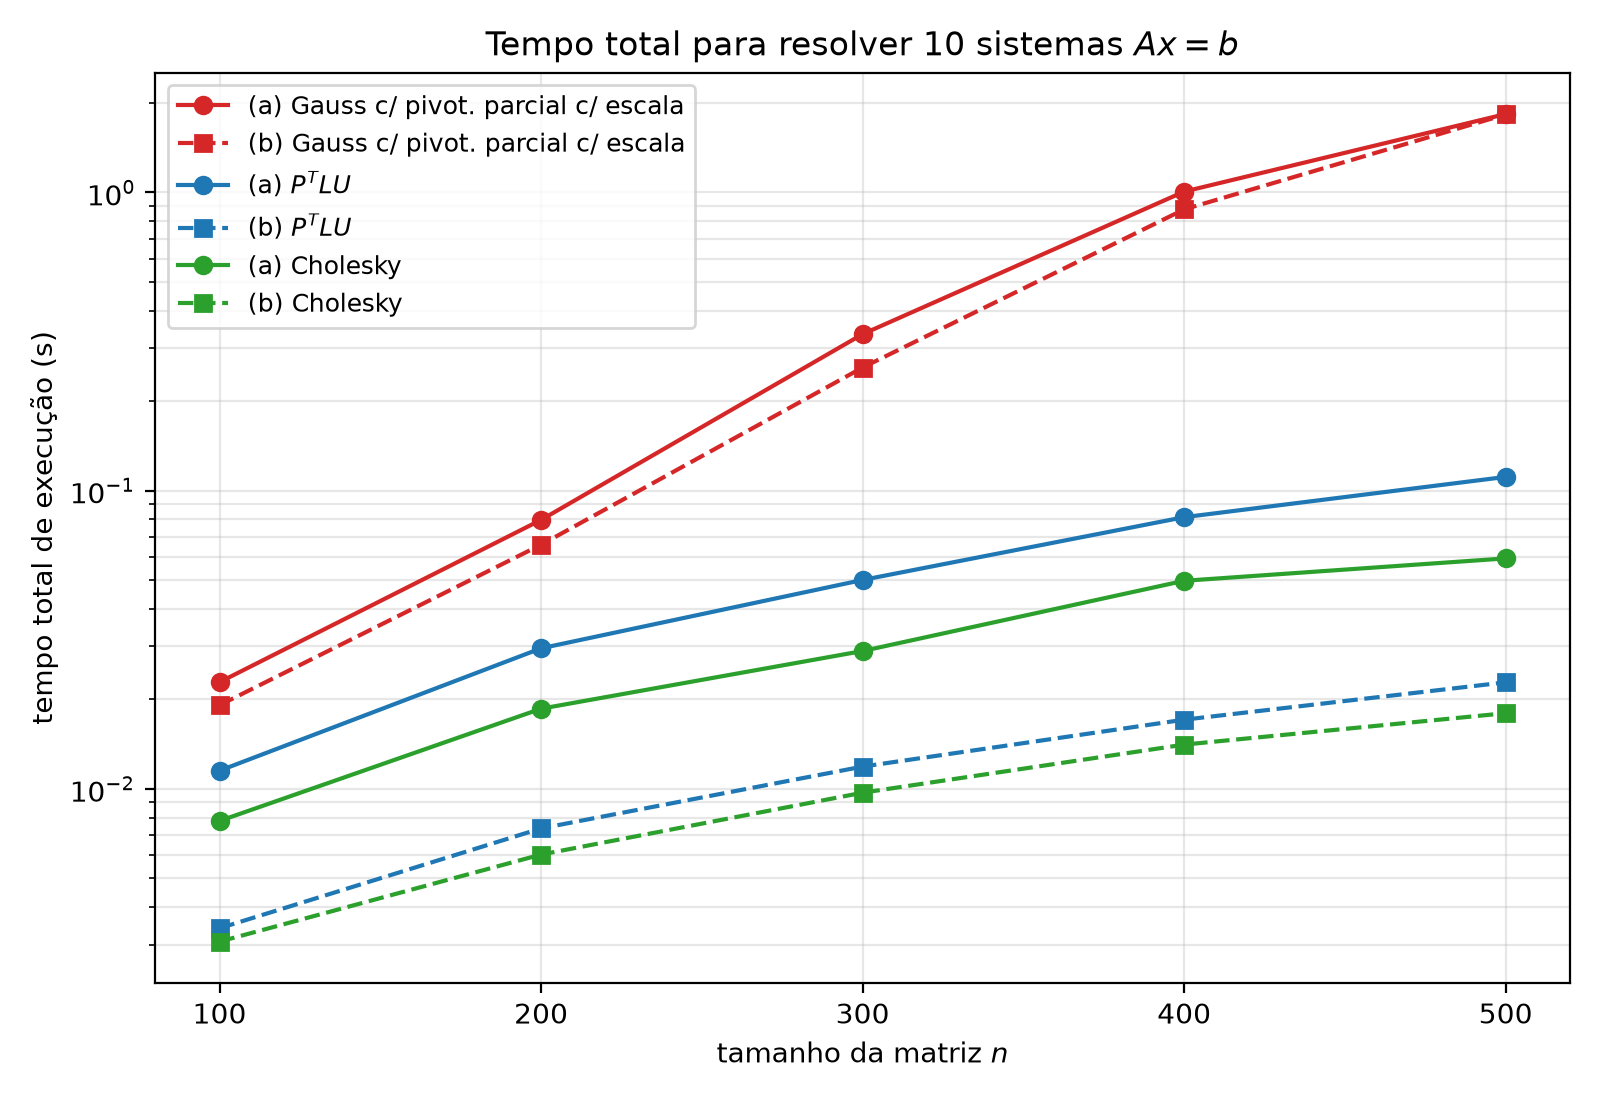
\includegraphics[width=0.62\textwidth]{q2_tempos_log.png}
\caption{Figura complementar, com os mesmos dados da Figura~1 e eixo vertical logarítmico (apenas para enxergar as
curvas pequenas). A figura pedida no enunciado, com as 6 curvas, é a Figura~1.}
\end{figure}

\subsection{Respostas e discussão}
\textbf{Item (a): o menor tempo foi o da decomposição de Cholesky}, para todos os valores de $n$.
Em $n=500$, $P\T LU$ levou $1{,}88$ vez o tempo de Cholesky, perto da razão teórica $2$
($\frac{n^3}{3}$ contra $\frac{n^3}{6}$).

\textbf{Item (b): o menor tempo também foi o de Cholesky}, para todos os $n$, com $P\T LU$ logo atrás e a
eliminação de Gauss muito atrás ($\approx 80$ vezes mais lenta que $P\T LU$ e $\approx 102$ vezes mais lenta que
Cholesky em $n=500$). Aqui aparece o efeito pedido no enunciado: Gauss paga $O(n^3/3)$ para \emph{cada} $b$, enquanto
as fatorações pagam $O(n^3)$ uma única vez e depois só $O(n^2)$ por vetor. Por isso as curvas (b) de $P\T LU$ e Cholesky
ficam bem abaixo das curvas (a), enquanto as duas curvas de Gauss praticamente coincidem (o mesmo trabalho é feito 10 vezes
nos dois itens). A diferença entre Cholesky e $P\T LU$ em (b) é menor ($1{,}27$ vez) porque as 10 substituições,
que custam o mesmo nos dois métodos, passam a pesar bastante no total.

\paragraph{Por que Gauss ficou tão mais lento que $P\T LU$ em (a), se o número de operações é o mesmo?}
A contagem de operações ($\approx n^3/3$ para ambos) não é a única coisa que define o tempo: a forma como o algoritmo
percorre a memória também conta. Na forma do \burden{Algoritmo 6.3}, cada etapa $i$ \emph{reescreve} toda a submatriz restante
$(n-i)\times(n-i)$ por uma atualização de posto~1 (no código, \texttt{np.outer} cria uma matriz temporária de ordem $n-i$
por etapa, e a subtração lê e grava a submatriz inteira), ou seja, cada entrada é lida e gravada $O(n)$ vezes.
Na forma de produto interno do \burden{Algoritmo 6.4} (e do 6.6), cada entrada de $L$ e $U$ é calculada uma única vez como
$a_{ij}-\sum_k l_{ik}u_{kj}$, isto é, por produtos escalares sobre fatores já prontos, com muito menos tráfego de memória.
É a mesma aritmética em outra ordem, e é exatamente por isso que bibliotecas profissionais reorganizam a eliminação
dessa forma. O mesmo efeito explica por que, em (b), a razão medida Gauss/$P\T LU$ em $n=500$ ($\approx 80$) é bem maior que a razão
teórica $\frac{10\,n^3/3}{n^3/3+10n^2}\approx 9{,}4$. Além disso, para $n\le500$ o tempo das fatorações ainda é dominado pelo custo fixo de cada
iteração do laço em Python: a inclinação medida entre $n=100$ e $n=500$ no gráfico log-log foi $\approx 2{,}7$--$2{,}8$ para
Gauss e apenas $\approx 1{,}1$--$1{,}4$ para $P\T LU$ e Cholesky (e não $3$); para $n$ maiores, a razão $n^3$
passa a dominar. Nada disso altera as conclusões: \emph{Cholesky foi o mais rápido nos dois itens}, como prevê a contagem
de operações, e em (b) as fatorações reaproveitadas vencem a eliminação por larga margem.

%==========================================================================
\section{Questão 3 --- Temperatura de equilíbrio numa placa circular}
%==========================================================================

\subsection*{(a) Sistema $t=Mt+b$ e $At=b$}
A \textbf{propriedade discreta do valor médio} (Anton \& Rorres, §10.11) afirma que, no equilíbrio, a temperatura num
ponto interior da malha é aproximadamente a \emph{média aritmética} das temperaturas dos quatro pontos vizinhos
(acima, abaixo, à esquerda, à direita). Ela é a discretização da equação de Laplace $u_{xx}+u_{yy}=0$: com a fórmula de
diferenças centradas de segunda ordem e espaçamento $h$,
\[
\frac{u_E-2u_P+u_W}{h^2}+\frac{u_N-2u_P+u_S}{h^2}=0\iff u_P=\tfrac14\,(u_N+u_S+u_E+u_W).
\]
Numerando $t_1$ (superior esquerdo), $t_2$ (superior direito), $t_3$ (inferior esquerdo) e $t_4$ (inferior direito), e
lembrando que o contorno vale $0$ na metade esquerda e $1$ na metade direita (figura do enunciado):
\begin{align*}
t_1&=\tfrac14\,(\underbrace{0}_{\text{cima}}+\underbrace{0}_{\text{esq.}}+t_2+t_3), &
t_2&=\tfrac14\,(\underbrace{1}_{\text{cima}}+\underbrace{1}_{\text{dir.}}+t_1+t_4),\\
t_3&=\tfrac14\,(\underbrace{0}_{\text{baixo}}+\underbrace{0}_{\text{esq.}}+t_1+t_4), &
t_4&=\tfrac14\,(\underbrace{1}_{\text{baixo}}+\underbrace{1}_{\text{dir.}}+t_2+t_3).
\end{align*}
Em forma matricial, $t=Mt+b$ com
\[
M=\frac14\begin{bmatrix}0&1&1&0\\1&0&0&1\\1&0&0&1\\0&1&1&0\end{bmatrix},\qquad
b=\begin{bmatrix}0\\[2pt] \tfrac12\\[2pt] 0\\[2pt] \tfrac12\end{bmatrix}.
\]
Como $t=Mt+b\iff (I-M)t=b$, o sistema é $At=b$ com
\[
A=I-M=\begin{bmatrix}1&-\frac14&-\frac14&0\\[2pt]-\frac14&1&0&-\frac14\\[2pt]-\frac14&0&1&-\frac14\\[2pt]0&-\frac14&-\frac14&1\end{bmatrix}.
\]
(No código, $M$ e $b$ são montados automaticamente a partir da lista de vizinhos de cada ponto.)
Observe que $A$ é simétrica, tem diagonal positiva e $1>\frac14+\frac14=R_i$: pelo teorema da Questão~1, já
\emph{esperamos} que $A$ seja PD, e o item (b) confirma isso algoritmicamente.

\subsection*{(b) Cholesky como teste de positividade}
\begin{proposicao}\label{prop:chol}
Seja $A$ simétrica. O Algoritmo 6.6 termina com todos os radicandos
$d_i=a_{ii}-\sum_{k<i}l_{ik}^2$ estritamente positivos se e somente se $A$ é positiva definida.
\end{proposicao}
\begin{proof}
($\Leftarrow$) Se $A$ é PD, cada submatriz principal dominante $A_k$ é PD e $\det A_k>0$ \burden{Teorema 6.25, p.~462}.
Por indução, se o algoritmo chegou à etapa $k$, então $A_k=L_kL_k\T$ e
$\det A_k=l_{11}^2\cdots l_{k-1,k-1}^2\,d_k$, de modo que $d_k=\det A_k/(l_{11}\cdots l_{k-1,k-1})^2>0$.
($\Rightarrow$) Se todos os $d_i>0$, obtemos $A=LL\T$ com $l_{ii}=\sqrt{d_i}>0$; $L\T$ é invertível e, para $x\neq0$,
$x\T Ax=x\T LL\T x=\|L\T x\|_2^2>0$. (É o conteúdo do \burden{Teorema 6.26 e Corolário 6.28, p.~463}.)
\end{proof}
\begin{sloppypar}\noindent \textbf{Adaptação feita} (\texttt{cholesky\_com\_teste}, que reaproveita as fórmulas de
\texttt{fatoracao\_cholesky} da Questão~2): (1) verifica-se a simetria (exigida pela Definição~6.22); (2) executa-se o
Algoritmo~6.6 e, se algum radicando $d_i$ não for estritamente positivo, devolve-se ``não é PD'' em vez de calcular a raiz
de um número não-positivo. Em ponto flutuante, ``$d_i>0$'' é testado com tolerância relativa ($d_i\le10^{-10}a_{ii}$ é tratado
como zero): sem ela, uma matriz apenas semidefinida (singular) pode gerar $d_i\approx10^{-17}>0$ por erro de arredondamento e ser
aceita como PD (ver a ilustração numérica da Questão~4). O custo do teste é o da própria fatoração. Como verificação, o detector responde
corretamente ``não PD'' para $\left(\begin{smallmatrix}1&2\\2&1\end{smallmatrix}\right)$ (autovalores $3$ e $-1$): $d_2=1-4=-3<0$.
Para exercitar o caminho alternativo, o sistema $\left(\begin{smallmatrix}1&2\\2&1\end{smallmatrix}\right)x=(3,3)\T$ é então resolvido
por $P\T LU$ e devolve $x=(1,1)\T$, como esperado.
\end{sloppypar}

\paragraph{Aplicação a $A=I-M$.} O teste retornou \textbf{$A$ positiva definida}; portanto o sistema foi resolvido por
Cholesky. Os fatores (exatos e numéricos) são
{\small\[L=\begin{bmatrix} 1&0&0&0\\ -\frac14&\frac{\sqrt{15}}{4}&0&0\\ -\frac14&-\frac{1}{4\sqrt{15}}&\sqrt{\frac{14}{15}}&0\\ 0&-\frac{1}{\sqrt{15}}&-\frac{4}{\sqrt{210}}&\sqrt{\frac67} \end{bmatrix} \approx \begin{bmatrix} 1&0&0&0\\ -0.25&0.9682&0&0\\ -0.25&-0.0645&0.9661&0\\ 0&-0.2582&-0.2760&0.9258 \end{bmatrix},\]}
com $d=(1,\ \tfrac{15}{16},\ \tfrac{14}{15},\ \tfrac67)$, todos positivos, e $\Vert{}LL\T-A\Vert{}_{\max}\approx2\times10^{-16}$.
Por exemplo, $l_{22}=\sqrt{1-(-\frac14)^2}=\frac{\sqrt{15}}{4}$ e
$l_{32}=\big(0-(-\frac14)(-\frac14)\big)/l_{22}=-\frac{1}{4\sqrt{15}}$.
Substituição progressiva $Ly=b$: $y\approx(0,\ 0.5164,\ 0.0345,\ 0.6944)\T$; regressiva $L\T t=y$:
\[\boxed{\,t_1=0.25,\quad t_2=0.75,\quad t_3=0.25,\quad t_4=0.75\,}\]
e $\Vert{}t-(Mt+b)\Vert{}_\infty\approx2\times10^{-16}$.

\paragraph{Conferência analítica.} A placa e o contorno são simétricos em relação ao eixo horizontal, logo
$t_1=t_3$ e $t_2=t_4$. A primeira equação dá $4t_1=t_2+t_1$, isto é, $t_2=3t_1$; a segunda dá
$4t_2=2+t_1+t_2$, isto é, $3t_2=2+t_1$. Então $9t_1=2+t_1$, logo $t_1=\frac14$ e $t_2=\frac34$, exatamente o resultado numérico.
Note ainda que $t_1+t_2=1$: trocar esquerda $\leftrightarrow$ direita troca $T\mapsto1-T$, como esperado fisicamente.

\subsection*{(c) Figura da placa}
\begin{figure}[H]\centering
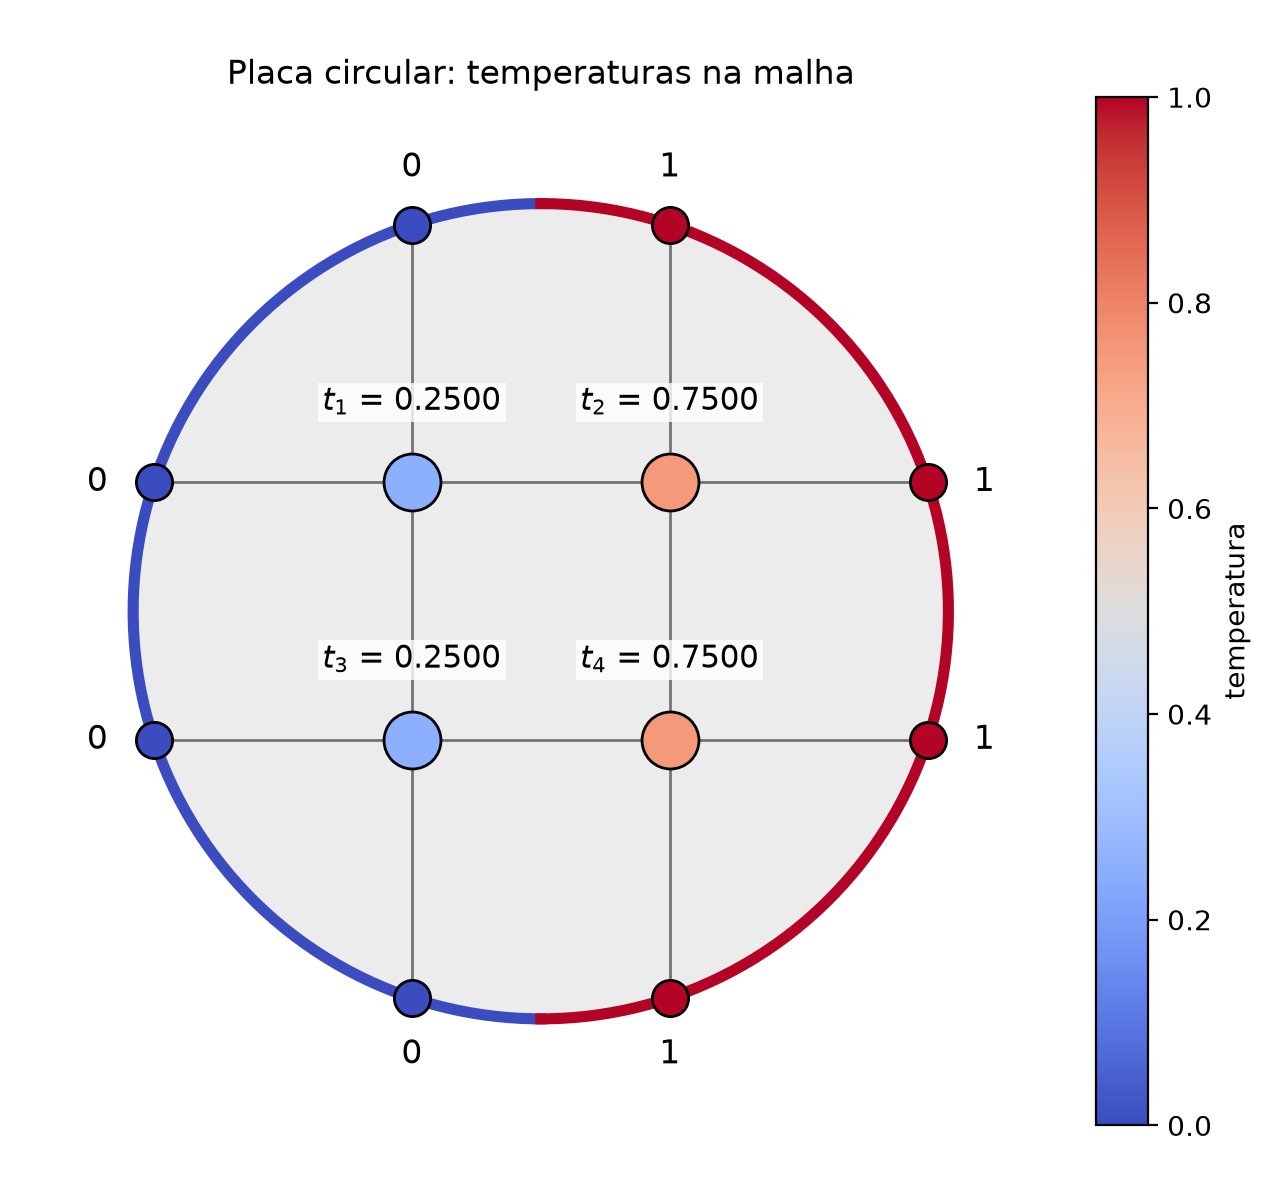
\includegraphics[width=0.62\textwidth]{q3_placa.png}
\caption{Malha sobre a placa: 8 pontos de contorno (0 à esquerda, 1 à direita) e 4 pontos interiores coloridos pela
temperatura calculada (escala \emph{coolwarm}). Os pontos de contorno foram colocados à mesma distância $h$ dos
interiores, de modo que a malha seja uniforme.}
\end{figure}

%==========================================================================
\section{Questão 4 --- Matriz de Gram $A=B\T B$}
%==========================================================================
Seja $B\in\R^{m\times n}$ e $A=B\T B\in\R^{n\times n}$. Note que $a_{ij}=\sum_{k=1}^m b_{ki}b_{kj}=\langle B_{:,i},B_{:,j}\rangle$
é o produto escalar entre as colunas $i$ e $j$ de $B$.

\subsection*{(a) $A$ é simétrica}
Usando $(XY)\T=Y\T X\T$ e $(X\T)\T=X$:
\[A\T=(B\T B)\T=B\T\,(B\T)\T=B\T B=A .\]
(Em coordenadas: $a_{ij}=\langle B_{:,i},B_{:,j}\rangle=\langle B_{:,j},B_{:,i}\rangle=a_{ji}$, pois o produto escalar é comutativo.)

\subsection*{(b) $A$ é positiva semidefinida}
Para qualquer $x\in\R^n$, seja $y=Bx\in\R^m$. Então, pela associatividade do produto de matrizes e pelo item (a),
\[x\T Ax=x\T B\T Bx=(Bx)\T(Bx)=y\T y=\sum_{k=1}^m y_k^2=\Vert{}Bx\Vert{}_2^2\;\ge\;0 ,\]
pois é uma soma de quadrados de números reais. Logo $A$ é positiva semidefinida. \qed

\paragraph{Quando $A$ é de fato positiva definida?} Pela conta acima, $x\T Ax=0\iff Bx=0$. Assim, $A$ é PD (no sentido da
\burden{Definição 6.22}) se e somente se $Bx=0$ só admite $x=0$, isto é, se as colunas de $B$ são linearmente
independentes (posto $n$, o que exige $m\ge n$). Se $m<n$, há $z\ne0$ com $Bz=0$ e então $z\T Az=0$: $A$ é apenas
semidefinida. Esse é o caso das \emph{equações normais} $B\T Bx=B\T y$ dos mínimos quadrados \burden{Seção 8.1}; não por acaso,
Cholesky criou sua fatoração justamente para resolver problemas de mínimos quadrados \burden{nota histórica, p.~464}.

\paragraph{Ilustração numérica (\texttt{questao4.py}).} Para $B$ aleatórias $5\times3$, $3\times3$ e $2\times4$,
obteve-se $\max\vert{}A-A\T\vert{}=0$ e $x\T Ax=\Vert{}Bx\Vert{}_2^2\ge0$ em $20\,000$ vetores sorteados. O teste de Cholesky da Questão~3
classificou $A$ como PD nos casos $5\times3$ e $3\times3$ (colunas independentes) e como \emph{não} PD no caso $2\times4$,
em que o programa encontrou $z\neq0$ com $Bz=0$ e $z\T Az\approx 10^{-17}$ (zero, a menos de arredondamento).
Para não depender de um único sorteio, o script repete o teste em $5\,000$ matrizes $B$ com $m<n$ ($A$ singular, apenas semidefinida):
o teste aceitou $A$ como PD em apenas $2$ casos ($0{,}04\%$), de matrizes numericamente quase singulares, em que o arredondamento impede
distinguir PD de semidefinida; sem a tolerância relativa seriam $693$ casos ($13{,}9\%$). Em outros $5\,000$ sorteios com $m\ge n$
(colunas independentes), o teste respondeu PD em todos.

%==========================================================================
\appendix
\section{Códigos}
%==========================================================================
\begin{sloppypar}
Execução dos scripts (na mesma pasta, pois \texttt{questao2.py} importa \texttt{questao1.py}, \texttt{questao3.py} importa
\texttt{questao2.py} e \texttt{questao4.py} importa \texttt{questao3.py}): \texttt{python questao1.py},
\texttt{python questao2.py} (gera \texttt{q2\_tempos.png}, \texttt{q2\_tempos\_log.png} e \texttt{q2\_resultados.json}),
\texttt{python questao3.py} (gera \texttt{q3\_placa.png}) e \texttt{python questao4.py}.
\end{sloppypar}

\subsection*{\texttt{questao1.py}}
\begin{lstlisting}
"""
Questão 1 — Gerador aleatório de matrizes positivas definidas.

Ideia (Teorema do enunciado + Burden, Def. 6.20 e Def. 6.22):
    Se A é simétrica, estritamente diagonal dominante e tem diagonal
    não-negativa, então A é positiva definida.

Algoritmo:
    1. Sorteia os elementos abaixo da diagonal a_ij ~ U(-1, 1), i > j.
    2. Espelha: a_ji = a_ij (garante A = A^T).
    3. Para cada linha i, define
          a_ii = sum_{j != i} |a_ij| + delta_i , delta_i ~ U(1, 2) (> 0)
       o que garante |a_ii| > sum_{j != i} |a_ij| (dominância estrita)
       e a_ii > 0 (diagonal positiva).

Só usamos o NumPy como "contêiner" de vetores/matrizes e para sortear números.
Nenhuma rotina de álgebra linear pronta (numpy.linalg, scipy) é usada.
"""

import numpy as np


def gerar_matriz_pd(n, rng=None, faixa=1.0, margem=(1.0, 2.0)):
    """Gera uma matriz n x n simétrica, estritamente diagonal dominante,
    com diagonal positiva (logo, positiva definida)."""
    if rng is None:
        rng = np.random.default_rng()
    A = np.zeros((n, n))
    # 1) parte estritamente inferior aleatória
    for i in range(1, n):
        A[i, :i] = rng.uniform(-faixa, faixa, size=i)
    # 2) simetria: A = L + L^T
    A = A + A.T
    # 3) diagonal: soma dos módulos fora da diagonal + folga positiva
    soma_fora = np.abs(A).sum(axis=1) # diagonal ainda é zero aqui
    delta = rng.uniform(margem[0], margem[1], size=n)
    for i in range(n):
        A[i, i] = soma_fora[i] + delta[i]
    return A


# ---------------------------------------------------------------- verificações
def eh_simetrica(A, tol=0.0):
    n = A.shape[0]
    for i in range(n):
        for j in range(i + 1, n):
            if abs(A[i, j] - A[j, i]) > tol:
                return False
    return True


def eh_estritamente_diagonal_dominante(A):
    n = A.shape[0]
    for i in range(n):
        soma = 0.0
        for j in range(n):
            if j != i:
                soma += abs(A[i, j])
        if not abs(A[i, i]) > soma:
            return False
    return True


def diagonal_nao_negativa(A):
    return all(A[i, i] >= 0 for i in range(A.shape[0]))


def menor_folga(A):
    """min_i ( a_ii - sum_{j!=i} |a_ij| ): quanto maior que zero, mais 'folgada'
    é a dominância diagonal. Pela demonstração, x^T A x >= menor_folga * ||x||^2."""
    n = A.shape[0]
    return min(A[i, i] - (np.abs(A[i]).sum() - abs(A[i, i])) for i in range(n))


def teste_empirico_forma_quadratica(A, amostras=20000, rng=None):
    """Sorteia vetores x != 0 e devolve o menor valor de x^T A x / x^T x."""
    if rng is None:
        rng = np.random.default_rng(0)
    n = A.shape[0]
    menor = np.inf
    for _ in range(amostras):
        x = rng.normal(size=n)
        q = x @ (A @ x)
        menor = min(menor, q / (x @ x))
    return menor


if __name__ == "__main__":
    rng = np.random.default_rng(2026)
    np.set_printoptions(precision=4, suppress=True, linewidth=120)

    for k, n in enumerate([3, 4, 5], start=1):
        A = gerar_matriz_pd(n, rng)
        print(f"===== Exemplo {k}: n = {n} =====")
        print(A)
        print(f" simétrica? {eh_simetrica(A)}")
        print(f" estritamente diag. dominante? {eh_estritamente_diagonal_dominante(A)}")
        print(f" diagonal não-negativa? {diagonal_nao_negativa(A)}")
        print(f" folga mínima min_i(a_ii - R_i) = {menor_folga(A):.4f}")
        print(f" min x^T A x / x^T x (20000 x aleatórios) = "
              f"{teste_empirico_forma_quadratica(A, rng=rng):.4f} (> 0)")
        print()
\end{lstlisting}

\subsection*{\texttt{questao2.py}}
\begin{lstlisting}
"""
Questão 2 — Eliminação Gaussiana com pivoteamento parcial com escala,
Decomposição P^T LU, Decomposição de Cholesky e substituições
(progressiva / regressiva) para resolver Ax = b; experimento de tempos.

Referências (Burden, Faires & Burden, Análise Numérica, 10ª ed.):
  * Algoritmo 6.1 (p. 403) — eliminação de Gauss + substituição regressiva
  * Algoritmo 6.3 (p. 417) — pivoteamento parcial com escala
  * Teorema 6.19 / Alg. 6.4 (pp. 448–450) e p. 452 — fatoração LU e A = P^T L U
  * Corolário 6.28 / Algoritmo 6.6 (pp. 463–464) — fatoração de Cholesky A = L L^T

Restrição da lista: "sem bibliotecas numéricas avançadas". O NumPy é usado
apenas como contêiner de vetores/matrizes e para operações elementares
(somas, produtos escalares, operações de linha). NÃO se usa numpy.linalg
nem scipy: todos os algoritmos estão escritos abaixo.

Uso:
    python questao2.py # roda o experimento completo (itens a, b, c)
"""

import json
import time

import numpy as np

from questao1 import gerar_matriz_pd


class MatrizSingular(Exception):
    pass


class NaoPositivaDefinida(Exception):
    pass


# =============================================================================
# Substituições (as "variações de substituição reversa")
# =============================================================================
def substituicao_progressiva(L, b, diagonal_unitaria=False):
    """Resolve L y = b, L triangular inferior (forward substitution).
    y_1 = b_1 / l_11 ; y_i = (b_i - sum_{j<i} l_ij y_j) / l_ii ."""
    n = L.shape[0]
    y = np.zeros(n)
    for i in range(n):
        s = b[i] - L[i, :i] @ y[:i]
        y[i] = s if diagonal_unitaria else s / L[i, i]
    return y


def substituicao_regressiva(U, y):
    """Resolve U x = y, U triangular superior (back substitution, Alg. 6.1 passos 8–9).
    x_n = y_n / u_nn ; x_i = (y_i - sum_{j>i} u_ij x_j) / u_ii ."""
    n = U.shape[0]
    x = np.zeros(n)
    for i in range(n - 1, -1, -1):
        if U[i, i] == 0:
            raise MatrizSingular("pivô nulo na substituição regressiva")
        x[i] = (y[i] - U[i, i + 1:] @ x[i + 1:]) / U[i, i]
    return x


def substituicao_regressiva_transposta(L, y):
    """Resolve L^T x = y usando apenas L (sem montar L^T):
    x_i = (y_i - sum_{j>i} l_ji x_j) / l_ii . (passos 9–10 após o Alg. 6.6)"""
    n = L.shape[0]
    x = np.zeros(n)
    for i in range(n - 1, -1, -1):
        x[i] = (y[i] - L[i + 1:, i] @ x[i + 1:]) / L[i, i]
    return x


# =============================================================================
# 1) Eliminação Gaussiana com pivoteamento parcial com escala (Alg. 6.3)
# =============================================================================
def fatores_de_escala(A):
    """s_i = max_j |a_ij| (Passo 1 do Alg. 6.3)."""
    s = np.abs(A).max(axis=1)
    if np.any(s == 0):
        raise MatrizSingular("linha nula: não existe solução única")
    return s


def eliminacao_gauss_escala(A, b):
    """Resolve Ax = b por eliminação de Gauss com pivoteamento parcial com escala.
    As trocas de linha são 'simuladas' com o vetor NLINHA, como no livro."""
    a = np.array(A, dtype=float) # cópia: não altera A
    bb = np.array(b, dtype=float)
    n = a.shape[0]
    s = fatores_de_escala(a)
    nlinha = np.arange(n) # NLINHA(i) = i

    for i in range(n - 1):
        # Passo 3: menor p >= i que maximiza |a(NLINHA(p), i)| / s(NLINHA(p))
        candidatas = nlinha[i:]
        razoes = np.abs(a[candidatas, i]) / s[candidatas]
        p = i + int(np.argmax(razoes))
        if a[nlinha[p], i] == 0:
            raise MatrizSingular("não existe solução única")
        # Passo 5: troca simulada
        if p != i:
            nlinha[i], nlinha[p] = nlinha[p], nlinha[i]
        piv = nlinha[i]
        abaixo = nlinha[i + 1:]
        # Passos 6–7: m_ji = a_ji / a_ii ; E_j <- E_j - m_ji E_i
        m = a[abaixo, i] / a[piv, i]
        a[abaixo, i:] -= np.outer(m, a[piv, i:])
        bb[abaixo] -= m * bb[piv]

    if a[nlinha[n - 1], n - 1] == 0:
        raise MatrizSingular("não existe solução única")
    # Substituição regressiva na ordem NLINHA (sistema triangular superior)
    return substituicao_regressiva(a[nlinha], bb[nlinha])


# =============================================================================
# 2) Decomposição P^T L U (PA = LU <=> A = P^T L U)
# =============================================================================
def fatoracao_ptlu(A, com_escala=True):
    """Fatoração de Doolittle (Alg. 6.4, l_ii = 1) com trocas de linhas.

    Usa as fórmulas do Alg. 6.4 em forma de produto interno:
        u_ij = a_ij - sum_{k<i} l_ik u_kj (linha i de U)
        l_ji = (a_ji - sum_{k<i} l_jk u_ki) / u_ii (coluna i de L)
    Antes de dividir por u_ii, escolhe-se o pivô na coluna i pelo critério do
    pivoteamento parcial com escala (Alg. 6.3) e trocam-se as linhas.

    Devolve (LU, perm): L (diagonal unitária, abaixo da diagonal) e U (diagonal
    e acima) guardadas na mesma matriz, e o vetor de permutação perm tal que
    P[i, perm[i]] = 1, ou seja, (PA)[i] = A[perm[i]] e PA = LU."""
    a = np.array(A, dtype=float)
    n = a.shape[0]
    perm = np.arange(n)
    s = fatores_de_escala(a) if com_escala else np.ones(n)

    for i in range(n):
        # candidatos a pivô: a_ji - sum_{k<i} l_jk u_ki , j = i..n-1
        a[i:, i] -= a[i:, :i] @ a[:i, i]
        p = i + int(np.argmax(np.abs(a[i:, i]) / s[i:]))
        if a[p, i] == 0:
            raise MatrizSingular("fatoração impossível: matriz singular")
        if p != i: # troca de linhas (inclui parte já calculada de L)
            a[[i, p]] = a[[p, i]]
            perm[[i, p]] = perm[[p, i]]
            s[[i, p]] = s[[p, i]]
        # linha i de U (colunas i+1..n-1)
        a[i, i + 1:] -= a[i, :i] @ a[:i, i + 1:]
        # coluna i de L (multiplicadores)
        a[i + 1:, i] /= a[i, i]
    return a, perm


def resolver_ptlu(LU, perm, b):
    """Ax = b com A = P^T L U: L y = P b (progressiva), U x = y (regressiva)."""
    pb = np.asarray(b, dtype=float)[perm]
    y = substituicao_progressiva(LU, pb, diagonal_unitaria=True)
    return substituicao_regressiva(LU, y)


def extrair_P_L_U(LU, perm):
    n = LU.shape[0]
    L = np.tril(LU, -1) + np.eye(n)
    U = np.triu(LU)
    P = np.zeros((n, n))
    P[np.arange(n), perm] = 1.0
    return P, L, U


# =============================================================================
# 3) Decomposição de Cholesky A = L L^T (Alg. 6.6)
# =============================================================================
def fatoracao_cholesky(A):
    """l_ii = sqrt(a_ii - sum_{k<i} l_ik^2)
       l_ji = (a_ji - sum_{k<i} l_jk l_ik) / l_ii , j > i."""
    A = np.asarray(A, dtype=float)
    n = A.shape[0]
    L = np.zeros((n, n))
    for i in range(n):
        d = A[i, i] - L[i, :i] @ L[i, :i]
        if d <= 0:
            raise NaoPositivaDefinida(f"pivô {d:.3e} <= 0 na etapa {i + 1}")
        L[i, i] = np.sqrt(d)
        L[i + 1:, i] = (A[i + 1:, i] - L[i + 1:, :i] @ L[i, :i]) / L[i, i]
    return L


def resolver_cholesky(L, b):
    """Ax = b com A = L L^T: L y = b (progressiva), L^T x = y (regressiva)."""
    y = substituicao_progressiva(L, b)
    return substituicao_regressiva_transposta(L, y)


# =============================================================================
# Experimento
# =============================================================================
def vetor_b_nao_nulo(n, rng):
    while True:
        b = rng.uniform(-10, 10, size=n)
        if np.any(b != 0):
            return b


def residuo(A, x, b):
    return float(np.max(np.abs(A @ x - b)))


def _mediana(v):
    v = sorted(v)
    return v[len(v) // 2]


def item_a(ns, reps, rng, repeticoes=5):
    """10 matrizes PD distintas e 10 vetores b: um sistema A_k x = b_k por par.
    Cada A_k é diferente, então os três métodos têm de processar A_k do zero.
    O tempo total (10 sistemas) é medido `repeticoes` vezes e guarda-se a mediana,
    para reduzir o ruído do sistema operacional."""
    tempos = {"Gauss": [], "PtLU": [], "Cholesky": []}
    for n in ns:
        As = [gerar_matriz_pd(n, rng) for _ in range(reps)]
        bs = [vetor_b_nao_nulo(n, rng) for _ in range(reps)]
        medidas = {"Gauss": [], "PtLU": [], "Cholesky": []}
        res_max = 0.0
        for _ in range(repeticoes):
            t0 = time.perf_counter()
            xs1 = [eliminacao_gauss_escala(A, b) for A, b in zip(As, bs)]
            t1 = time.perf_counter()
            xs2 = []
            for A, b in zip(As, bs):
                LU, perm = fatoracao_ptlu(A) # cada A é nova: precisa fatorar
                xs2.append(resolver_ptlu(LU, perm, b))
            t2 = time.perf_counter()
            xs3 = []
            for A, b in zip(As, bs):
                L = fatoracao_cholesky(A)
                xs3.append(resolver_cholesky(L, b))
            t3 = time.perf_counter()
            medidas["Gauss"].append(t1 - t0)
            medidas["PtLU"].append(t2 - t1)
            medidas["Cholesky"].append(t3 - t2)
        for A, b, x1, x2, x3 in zip(As, bs, xs1, xs2, xs3):
            res_max = max(res_max, residuo(A, x1, b), residuo(A, x2, b), residuo(A, x3, b))
        t = {k: _mediana(v) for k, v in medidas.items()}
        for k in tempos:
            tempos[k].append(t[k])
        print(f"(a) n={n:4d} Gauss={t['Gauss']:.4f}s PtLU={t['PtLU']:.4f}s "
              f"Cholesky={t['Cholesky']:.4f}s max||Ax-b||_inf={res_max:.2e}")
    return tempos


def item_b(ns, reps, rng, repeticoes=5):
    """1 matriz PD e 10 vetores b. Gauss refaz a eliminação a cada b;
    P^T LU e Cholesky fatoram UMA vez e reaproveitam a fatoração
    (só as substituições, O(n^2), são repetidas para cada b)."""
    tempos = {"Gauss": [], "PtLU": [], "Cholesky": []}
    for n in ns:
        A = gerar_matriz_pd(n, rng)
        bs = [vetor_b_nao_nulo(n, rng) for _ in range(reps)]
        medidas = {"Gauss": [], "PtLU": [], "Cholesky": []}
        for _ in range(repeticoes):
            t0 = time.perf_counter()
            xs1 = [eliminacao_gauss_escala(A, b) for b in bs]
            t1 = time.perf_counter()

            LU, perm = fatoracao_ptlu(A) # fatora uma única vez
            xs2 = [resolver_ptlu(LU, perm, b) for b in bs]
            t2 = time.perf_counter()

            L = fatoracao_cholesky(A) # fatora uma única vez
            xs3 = [resolver_cholesky(L, b) for b in bs]
            t3 = time.perf_counter()
            medidas["Gauss"].append(t1 - t0)
            medidas["PtLU"].append(t2 - t1)
            medidas["Cholesky"].append(t3 - t2)

        res_max = 0.0
        for b, x1, x2, x3 in zip(bs, xs1, xs2, xs3):
            res_max = max(res_max, residuo(A, x1, b), residuo(A, x2, b), residuo(A, x3, b))
        t = {k: _mediana(v) for k, v in medidas.items()}
        for k in tempos:
            tempos[k].append(t[k])
        print(f"(b) n={n:4d} Gauss={t['Gauss']:.4f}s PtLU={t['PtLU']:.4f}s "
              f"Cholesky={t['Cholesky']:.4f}s max||Ax-b||_inf={res_max:.2e}")
    return tempos


def plotar(ns, ta, tb, arquivo="q2_tempos.png", log=False):
    import matplotlib
    matplotlib.use("Agg")
    import matplotlib.pyplot as plt

    cores = {"Gauss": "tab:red", "PtLU": "tab:blue", "Cholesky": "tab:green"}
    rotulo = {"Gauss": "Gauss c/ pivot. parcial c/ escala",
              "PtLU": r"$P^TLU$", "Cholesky": "Cholesky"}
    fig, ax = plt.subplots(figsize=(8, 5.5))
    for k in ["Gauss", "PtLU", "Cholesky"]:
        ax.plot(ns, ta[k], "-o", color=cores[k], label=f"(a) {rotulo[k]}")
        ax.plot(ns, tb[k], "--s", color=cores[k], label=f"(b) {rotulo[k]}")
    ax.set_xlabel("tamanho da matriz $n$")
    ax.set_ylabel("tempo total de execução (s)")
    ax.set_title("Tempo total para resolver 10 sistemas $Ax=b$")
    ax.set_xticks(ns)
    if log:
        ax.set_yscale("log")
    ax.grid(alpha=0.3, which="both")
    ax.legend(fontsize=9)
    fig.tight_layout()
    fig.savefig(arquivo, dpi=200)
    plt.close(fig)


def demonstracao_pequena():
    """Mostra os três métodos num sistema 4x4 e confere que A = P^T L U e A = L L^T."""
    rng = np.random.default_rng(1)
    A = gerar_matriz_pd(4, rng)
    b = vetor_b_nao_nulo(4, rng)
    np.set_printoptions(precision=5, suppress=True)
    print("A =\n", A, "\nb =", b)
    print("Gauss (escala):", eliminacao_gauss_escala(A, b))
    LU, perm = fatoracao_ptlu(A)
    P, L, U = extrair_P_L_U(LU, perm)
    print("P^T LU :", resolver_ptlu(LU, perm, b),
          " ||P^T L U - A||_max =", np.abs(P.T @ L @ U - A).max())
    Lc = fatoracao_cholesky(A)
    print("Cholesky :", resolver_cholesky(Lc, b),
          " ||L L^T - A||_max =", np.abs(Lc @ Lc.T - A).max())
    print()


if __name__ == "__main__":
    demonstracao_pequena()

    ns = [100, 200, 300, 400, 500]
    reps = 10
    rng = np.random.default_rng(12345)

    # aquecimento (evita que a 1ª medição inclua custos de inicialização)
    _A = gerar_matriz_pd(50, rng); _b = vetor_b_nao_nulo(50, rng)
    eliminacao_gauss_escala(_A, _b); resolver_ptlu(*fatoracao_ptlu(_A), _b)
    resolver_cholesky(fatoracao_cholesky(_A), _b)

    ta = item_a(ns, reps, rng)
    print()
    tb = item_b(ns, reps, rng)

    with open("q2_resultados.json", "w") as f:
        json.dump({"n": ns, "a": ta, "b": tb}, f, indent=2)

    plotar(ns, ta, tb, "q2_tempos.png")
    plotar(ns, ta, tb, "q2_tempos_log.png", log=True)

    for item, t in (("a", ta), ("b", tb)):
        totais = {k: sum(v) for k, v in t.items()}
        venc = [min(t, key=lambda k: t[k][i]) for i in range(len(ns))]
        print(f"\nItem ({item}) — método mais rápido em cada n: "
              + ", ".join(f"n={n}: {m}" for n, m in zip(ns, venc)))
        print(f" tempos somados: " + ", ".join(f"{k}={v:.3f}s" for k, v in totais.items()))
\end{lstlisting}

\subsection*{\texttt{questao3.py}}
\begin{lstlisting}
"""
Questão 3 — Temperatura de equilíbrio numa placa circular (Anton & Rorres, §10.11).

Malha: 4 pontos interiores t1 (sup. esq.), t2 (sup. dir.), t3 (inf. esq.),
t4 (inf. dir.) e 8 pontos de contorno: temperatura 0 na metade esquerda da
circunferência e 1 na metade direita.

Propriedade discreta do valor médio: a temperatura num ponto interior é a média
das temperaturas nos 4 vizinhos (cima, baixo, esquerda, direita).
Isso dá t = M t + b -> (I - M) t = b -> A t = b.

Item (b): Cholesky "adaptado" — além de fatorar, decide se A é positiva definida
(Burden, Teorema 6.26 / Corolário 6.28: A simétrica é PD <=> a fatoração
A = L L^T existe com l_ii > 0, i.e., todos os radicandos são > 0).
"""

import numpy as np

from questao2 import (resolver_ptlu, fatoracao_ptlu, substituicao_progressiva,
                      substituicao_regressiva_transposta)


# ----------------------------------------------------------------------------- (a)
def montar_sistema():
    """Monta M e b a partir da vizinhança de cada ponto interior.
    Vizinhos do tipo ('t', k) são incógnitas; ('c', valor) são pontos de contorno."""
    vizinhos = {
        # ponto: cima baixo esquerda direita
        0: [("c", 0.0), ("t", 2), ("c", 0.0), ("t", 1)], # t1
        1: [("c", 1.0), ("t", 3), ("t", 0), ("c", 1.0)], # t2
        2: [("t", 0), ("c", 0.0), ("c", 0.0), ("t", 3)], # t3
        3: [("t", 1), ("c", 1.0), ("t", 2), ("c", 1.0)], # t4
    }
    M = np.zeros((4, 4))
    b = np.zeros(4)
    for i, viz in vizinhos.items():
        for tipo, v in viz:
            if tipo == "t":
                M[i, v] += 0.25
            else:
                b[i] += 0.25 * v
    return M, b


# ----------------------------------------------------------------------------- (b)
def cholesky_com_teste(A, tol_sim=1e-12, tol_pd=1e-10):
    """Algoritmo 6.6 (Cholesky) adaptado.
    Devolve (eh_pd, L). eh_pd = False se A não for simétrica ou se algum
    radicando d_i = a_ii - sum_k l_ik^2 não for estritamente positivo
    (nesse caso L = None).

    Em ponto flutuante, "d_i > 0" é testado com tolerância relativa: d_i <= tol_pd * a_ii
    é tratado como zero. Sem isso, uma matriz apenas semidefinida (singular) pode
    produzir d_i ~ 1e-17 > 0 por erro de arredondamento e ser aceita como PD."""
    A = np.asarray(A, dtype=float)
    n = A.shape[0]
    # 1) PD (no sentido do Burden, Def. 6.22) exige simetria
    for i in range(n):
        for j in range(i + 1, n):
            if abs(A[i, j] - A[j, i]) > tol_sim:
                return False, None
    # 2) fatoração; falha <=> A não é PD
    L = np.zeros((n, n))
    for i in range(n):
        d = A[i, i] - L[i, :i] @ L[i, :i]
        if d <= tol_pd * abs(A[i, i]):
            return False, None
        L[i, i] = np.sqrt(d)
        L[i + 1:, i] = (A[i + 1:, i] - L[i + 1:, :i] @ L[i, :i]) / L[i, i]
    return True, L


def resolver(A, b):
    eh_pd, L = cholesky_com_teste(A)
    if eh_pd:
        y = substituicao_progressiva(L, b)
        t = substituicao_regressiva_transposta(L, y)
        return t, "Cholesky", L
    LU, perm = fatoracao_ptlu(A)
    return resolver_ptlu(LU, perm, b), "P^T LU", None


# ----------------------------------------------------------------------------- (c)
def desenhar(t, arquivo="q3_placa.png"):
    import matplotlib
    matplotlib.use("Agg")
    import matplotlib.pyplot as plt
    from matplotlib.patches import Circle

    h = 1.0 # espaçamento da malha
    c = h / 2 # pontos interiores em (±h/2, ±h/2)
    yb = c + h # contorno a uma distância h dos interiores
    R = np.hypot(c, yb) # raio do disco que passa pelos 8 pontos

    interiores = {"$t_1$": (-c, c), "$t_2$": (c, c), "$t_3$": (-c, -c), "$t_4$": (c, -c)}
    contorno = [(-c, yb, 0), (c, yb, 1), (-yb, c, 0), (yb, c, 1),
                (-yb, -c, 0), (yb, -c, 1), (-c, -yb, 0), (c, -yb, 1)]

    cmap = plt.get_cmap("coolwarm")
    fig, ax = plt.subplots(figsize=(6.4, 6))
    ax.add_patch(Circle((0, 0), R, facecolor="#ececec", edgecolor="0.25", lw=1.5, zorder=0))
    # metades do contorno com a cor da temperatura
    th = np.linspace(np.pi / 2, 3 * np.pi / 2, 200)
    ax.plot(R * np.cos(th), R * np.sin(th), color=cmap(0.0), lw=4, zorder=1)
    ax.plot(-R * np.cos(th), R * np.sin(th), color=cmap(1.0), lw=4, zorder=1)
    # linhas da malha
    for v in (-c, c):
        ax.plot([v, v], [-yb, yb], color="0.45", lw=1, zorder=1)
        ax.plot([-yb, yb], [v, v], color="0.45", lw=1, zorder=1)

    for x, y, T in contorno:
        ax.scatter(x, y, s=170, c=[T], cmap=cmap, vmin=0, vmax=1,
                   edgecolors="k", zorder=3)
        dx, dy = 0.22 * np.sign(x) * (abs(x) > c), 0.22 * np.sign(y) * (abs(y) > c)
        ax.text(x + dx, y + dy, f"{T:g}", ha="center", va="center", fontsize=12)

    for (nome, (x, y)), T in zip(interiores.items(), t):
        sc = ax.scatter(x, y, s=420, c=[T], cmap=cmap, vmin=0, vmax=1,
                        edgecolors="k", zorder=3)
        ax.text(x, y + 0.28, f"{nome} = {T:.4f}", ha="center", fontsize=11,
                bbox=dict(facecolor="white", edgecolor="none", alpha=0.8, pad=1.5))

    cb = fig.colorbar(sc, ax=ax, fraction=0.046, pad=0.04)
    cb.set_label("temperatura")
    ax.set_aspect("equal")
    ax.set_xlim(-R - 0.4, R + 0.4)
    ax.set_ylim(-R - 0.4, R + 0.4)
    ax.axis("off")
    ax.set_title("Placa circular: temperaturas na malha")
    fig.tight_layout()
    fig.savefig(arquivo, dpi=200)
    plt.close(fig)


if __name__ == "__main__":
    np.set_printoptions(precision=4, suppress=True)
    M, b = montar_sistema()
    A = np.eye(4) - M
    print("M =\n", M, "\nb =", b, "\nA = I - M =\n", A)

    eh_pd, L = cholesky_com_teste(A)
    print("\nA é positiva definida?", eh_pd)
    t, metodo, L = resolver(A, b)
    if L is not None:
        print("L (Cholesky) =\n", L)
        print("||L L^T - A||_max =", np.abs(L @ L.T - A).max())
    print(f"\nTemperaturas (resolvido por {metodo}):")
    for k, v in enumerate(t, start=1):
        print(f" t{k} = {v:.6f}")
    print("Verificação: ||t - (M t + b)||_inf =", np.abs(t - (M @ t + b)).max())

    # contra-exemplo: o teste detecta uma matriz simétrica NÃO PD
    B = np.array([[1.0, 2.0], [2.0, 1.0]])
    print("\nTeste do detector com B = [[1,2],[2,1]] (autovalores 3 e -1):",
          cholesky_com_teste(B)[0])

    # caminho alternativo: matriz simétrica NÃO PD é resolvida por P^T LU
    c = np.array([3.0, 3.0])
    x, metodo, _ = resolver(B, c)
    print(f"Sistema B x = {c} (B não PD) resolvido por {metodo}: x = {x} (esperado [1, 1])")

    desenhar(t)
    print("\nFigura salva em q3_placa.png")
\end{lstlisting}

\subsection*{\texttt{questao4.py}}
\begin{lstlisting}
"""
Questão 4 (teórica) — Matriz de Gram A = B^T B.

A demonstração está no relatório. Este script apenas ILUSTRA numericamente
as duas propriedades para matrizes B aleatórias de vários formatos:
  (a) A = A^T
  (b) x^T A x = ||Bx||_2^2 >= 0 para todo x
Também mostra o caso m < n, em que A é apenas semidefinida (existe x != 0 com
Bx = 0, logo x^T A x = 0), e usa o Cholesky com teste da questão 3 para mostrar
que, quando B tem colunas linearmente independentes, A é de fato definida positiva.
"""

import numpy as np

from questao3 import cholesky_com_teste


def gram(B):
    m, n = B.shape
    A = np.zeros((n, n))
    for i in range(n):
        for j in range(n):
            A[i, j] = B[:, i] @ B[:, j] # a_ij = <coluna i, coluna j>
    return A


def vetor_no_nucleo(B):
    """Para B (m x n) com m < n, encontra x != 0 com Bx = 0 por eliminação
    de Gauss (forma escalonada) — sem bibliotecas de álgebra linear."""
    a = np.array(B, dtype=float)
    m, n = a.shape
    pivos, lin = [], 0
    for col in range(n):
        if lin == m:
            break
        p = lin + int(np.argmax(np.abs(a[lin:, col])))
        if abs(a[p, col]) < 1e-12:
            continue
        a[[lin, p]] = a[[p, lin]]
        a[lin] /= a[lin, col]
        for r in range(m):
            if r != lin:
                a[r] -= a[r, col] * a[lin]
        pivos.append(col)
        lin += 1
    livre = next(c for c in range(n) if c not in pivos)
    x = np.zeros(n)
    x[livre] = 1.0
    for r, c in enumerate(pivos):
        x[c] = -a[r, livre]
    return x


if __name__ == "__main__":
    rng = np.random.default_rng(4)
    for (m, n) in [(5, 3), (3, 3), (2, 4)]:
        B = rng.normal(size=(m, n))
        A = gram(B)
        sim = np.abs(A - A.T).max()
        menor = min((x @ A @ x) for x in rng.normal(size=(20000, n)))
        print(f"B {m}x{n}: max|A - A^T| = {sim:.1e} "
              f"min x^T A x (20000 x) = {menor:.4e} "
              f"Cholesky diz PD? {cholesky_com_teste(A)[0]}")
        x = rng.normal(size=n)
        print(f" conferindo x^T A x = ||Bx||^2: {x @ A @ x:.6f} = {(B @ x) @ (B @ x):.6f}")
        if m < n:
            z = vetor_no_nucleo(B)
            print(f" m < n: z = {np.round(z, 4)} tem Bz = {np.round(B @ z, 12)} "
                  f"e z^T A z = {z @ A @ z:.1e} (zero, a menos de arredondamento) -> A é só semidefinida")

    # robustez do teste de Cholesky (Questão 3) sobre muitas matrizes de Gram:
    #   m < n  -> A é singular (só semidefinida): o teste nunca deve dizer "PD";
    #   m >= n -> colunas independentes (com prob. 1): o teste sempre deve dizer "PD".
    rng2 = np.random.default_rng(2026)
    tentativas = 5000
    pd_com_m_menor, pd_com_m_maior = 0, 0
    for _ in range(tentativas):
        n = int(rng2.integers(3, 8))
        m = int(rng2.integers(1, n))        # 1 <= m < n
        pd_com_m_menor += cholesky_com_teste(gram(rng2.normal(size=(m, n))))[0]
        m = int(rng2.integers(n, n + 4))    # m >= n
        pd_com_m_maior += cholesky_com_teste(gram(rng2.normal(size=(m, n))))[0]
    print(f"\n{tentativas} sorteios com m < n : teste disse PD em {pd_com_m_menor} (esperado 0)")
    print(f"{tentativas} sorteios com m >= n: teste disse PD em {pd_com_m_maior} (esperado {tentativas})")
\end{lstlisting}

\end{document}